\documentclass[../mathNotesPreamble]{subfiles}
\begin{document}
%\relscale{1.4} %TODO
\section{15.1: Graphs and Level Curves}

  In the previous chapter, we considered functions of the form 
    \[\vecr(t)=\bracket{f(t),\,g(t),\,h(t)},\]
  which have one independent variable $t$ and three dependent variables $f(t)$, $g(t)$, and $h(t)$. In this chapter, we consider functions of the form
    \[x_\npo=f(x_1,x_2,\dots,x_n),\]
  where we have multiple independent variables $x_1,\, x_2,\dots,\,x_n$ and one single dependent variable $x_\npo$. We begin with functions of two variables:
    \[z=f(x,y).\]

  \vspace*{\stretch{1}}
  \begin{defn*}[Function, Domain, and Range with 2 Independent Variables]
    A \textbf{function} $z=f(x,y)$ assigns to each point $(x,y)$ in a set $D$ in $\bbr^2$ a unique real number $z$ in a subset of $\bbr$. The set $D$ is the \textbf{domain} of $f$. The \textbf{range} of $f$ is the set of real numbers $z$ that are assumed as the points $(x,y)$ vary over the domain.
  \end{defn*}

  \begin{center}
    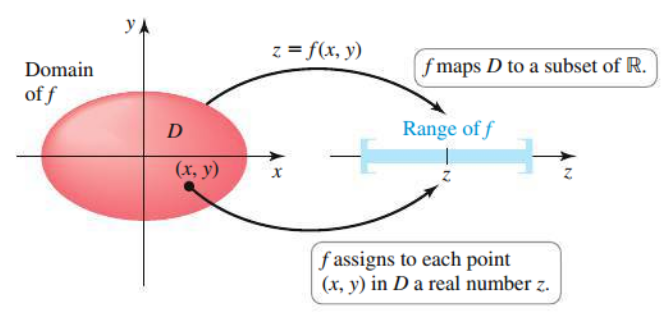
\includegraphics[width=0.7\linewidth]{../images/briggs_15_01/fig15_01}
  \end{center}
  \pagebreak

  \begin{ex*}
    Find the domain of the following functions:
  \end{ex*}
  \begin{tasks}[after-item-skip=\stretch{1}, label=](2)
    \task $\ds f(x,y)=\frac{1}{xy+2}$
    \task $\ds g(x,y)=\sqrt{108-3x^2-3y^2}$
    \task $\ds h(x,y)=\log_{2}\parens{x^3-y^{1/3}}$
    \task $\ds j(x,y)=\frac{1}{\sqrt{x^2+y^2-16}}$
  \end{tasks}
  \vspace*{\stretch{1}}
  \pagebreak

  \begin{ex*}
    Roughly graph the following functions:
  \end{ex*}
  \begin{tasks}[after-item-skip=\stretch{1}, label=](1)
    \task $\ds f(x,y)=-4x+3y-10$
    \task $\ds g(x,y)=x^2+y^2+4$
    \task $\ds h(x,y)=\sqrt{4+x^2+y^2}$
  \end{tasks}
  \vspace*{\stretch{1}}
  \pagebreak

  \textbf{Level Curves:}

  A \textbf{contour curve} is formed by tracing a three-dimensional surface at a constant height. A \textbf{level curve} is formed when a contour curve is projected to the $xy$-plane.
  \vspace*{\stretch{1}}
  \begin{center}
    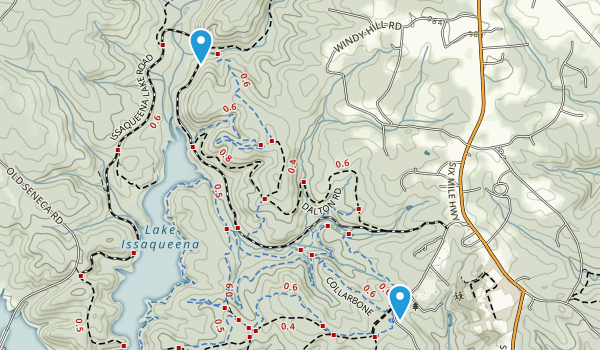
\includegraphics[width=0.75\linewidth]{../images/cuExperForestTopoMap}
  \end{center}
  \vspace*{\stretch{1}}

  \begin{center}
    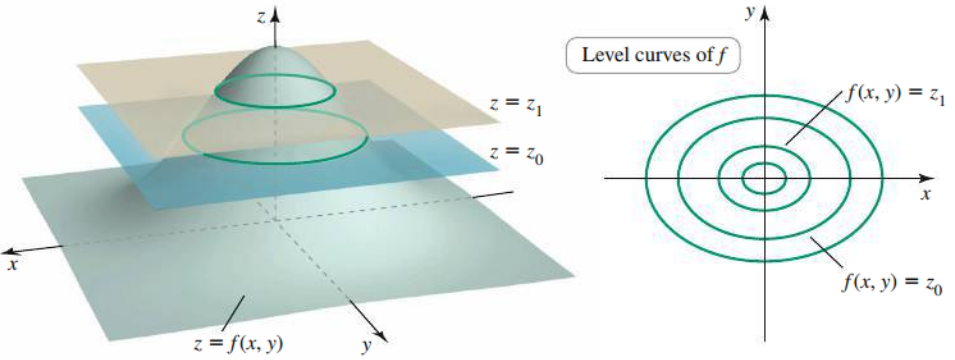
\includegraphics[width=0.8\linewidth]{../images/briggs_15_01/fig15_10}
  \end{center}
  \pagebreak

  \begin{ex*}
    Find the level curves of the following functions:
  \end{ex*}
  \begin{tasks}[after-item-skip=\stretch{1}, label=](1)
    \task $f(x,y)=y-x^2-1$
    \task $g(x,y)=e^{-x^2-y^2}$
    \task $h(x,y)=x^2+y^2$
  \end{tasks}
  \vspace*{\stretch{1}}
  \pagebreak

  \textbf{Applications of Functions of Two Variables:}
  \begin{ex*}
    \textbf{A probability function of two variables:} Suppose on a particular day, the fraction of students on campus infected with COVID-19 is $r$, where $0\leq r\leq 1$. If you have $n$ random (possibly repeated) encounters with students during the day, the probability of meeting \textit{at least} one infected person is $p(n,r)=1-(1-r)^n$. 
  \end{ex*}
  \begin{center}
    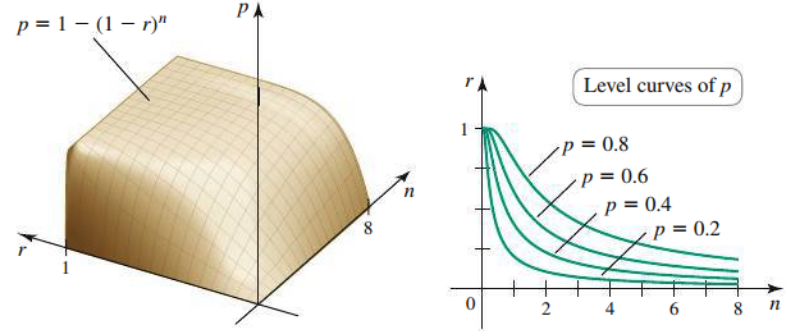
\includegraphics[width=0.75\linewidth]{../images/briggs_15_01/fig15_15}
  \end{center}
  \vspace*{\stretch{1}}

  \textbf{Functions of More than Two Variables:}
  
  \begin{center}
    \renewcommand{\arraystretch}{1.35}
    \begin{tabular}{@{}CR@{$=$}LR@{$=$}LL@{}}
      \toprule
      \lnret[c]{\textbf{Number of}\\ \textbf{Independent}\\ \textbf{Variables}}& \multicolumn{2}{c}{\textbf{Explicit Form}}& \multicolumn{2}{c}{\textbf{Implicit Form}}& \lnret[c]{\textbf{Graph Resides}\\ \textbf{In...}}\\
      1& y &f(x)& F(x,y) &0 &\bbr^2 (xy-\textnormal{plane})\\
      2& z &f(x,y)& F(x,y,z) &0 &\bbr^3 (xyz-\textnormal{space})\\
      3& w &f(x,y,z)& F(x,y,z,w) &0 &\bbr^4\\
      n& x_\npo& f(x_1,x_2,\dots,x_n)& F(x_1, x_2,\dots, x_n, x_\npo) &0 &\bbr^\npo\\\bottomrule
    \end{tabular}
  \end{center}

  \pagebreak
  \begin{defn*}[Function, Domain, and Range with $n$ Independent Variables]
    The \textbf{function} $x_\npo=f(x_1,x_2,\dots,x_n)$ assigns a unique real number $x_\npo$ to each point $(x_1,x_2,\dots,x_n)$ in a set $D$ in $\bbr^4$. The set $D$ is the \textbf{domain} of $f$. The \textbf{range} is the set of real numbers $x_\npo$ that are assumed as the points $(x_1,x_2,\dots,x_n)$ vary over the domain.
  \end{defn*}

  \begin{ex*}
    Find the domain of the following functions:
  \end{ex*}
  \begin{tasks}[after-item-skip=\stretch{1}, label=](1)
    \task $f(x,y,z)=4xyz-2xz+5yz$
    \task $f(x,y,z)=\sqrt{x^2+y^2+z^2-9}$
  \end{tasks}
  \vspace*{\stretch{1}}
  \pagebreak

  \textbf{Graphs of Functions of More Than Two Variables:}

  The idea of level curves can be extended to \textbf{level surfaces}. Level surfaces can be used to represent functions of three variables:
  \begin{center}
    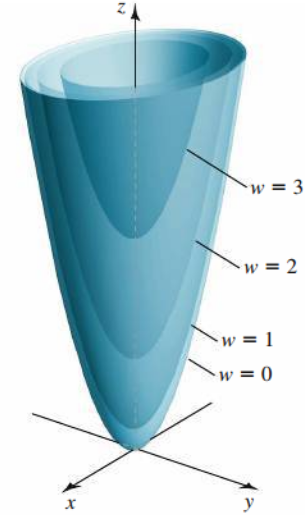
\includegraphics[width=0.25\linewidth]{../images/briggs_15_01/fig15_17}
  \end{center}
  \vspace*{\stretch{1}}

  \begin{center}
    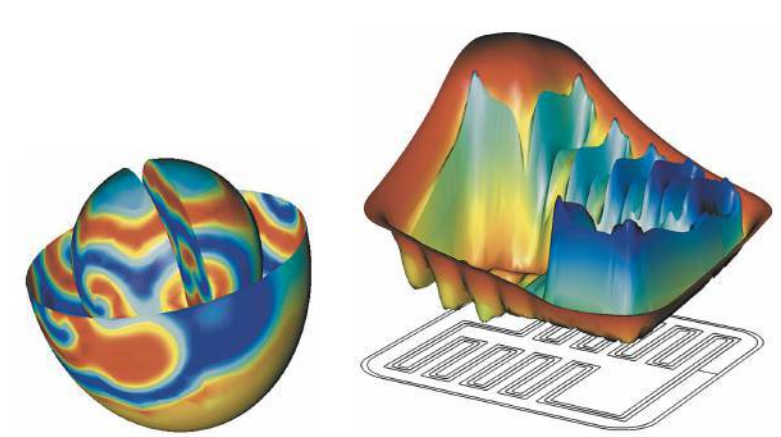
\includegraphics[width=0.85\linewidth]{../images/briggs_15_01/fig15_18}
  \end{center}

  \pagebreak
  
\end{document}